% Copyright 2015-2016 Dan Foreman-Mackey and the co-authors listed below.

\documentclass[manuscript, letterpaper]{aastex6}

\pdfoutput=1

\include{vc}
\usepackage{microtype}

\usepackage{url}
\usepackage{amssymb,amsmath}
\usepackage{natbib}
\usepackage{multirow}
\bibliographystyle{aasjournal}

% ----------------------------------- %
% start of AASTeX mods by DWH and DFM %
% ----------------------------------- %

\setlength{\voffset}{0in}
\setlength{\hoffset}{0in}
\setlength{\textwidth}{6in}
\setlength{\textheight}{9in}
\setlength{\headheight}{0ex}
\setlength{\headsep}{\baselinestretch\baselineskip} % this is 2 lines in ``manuscript''
\setlength{\footnotesep}{0in}
\setlength{\topmargin}{-\headsep}
\setlength{\oddsidemargin}{0.25in}
\setlength{\evensidemargin}{0.25in}

\linespread{0.54} % close to 10/13 spacing in ``manuscript''
\setlength{\parindent}{0.54\baselineskip}
\hypersetup{colorlinks = false}
\makeatletter % you know you are living your life wrong when you need to do this
\long\def\frontmatter@title@above{
\vspace*{-\headsep}\vspace*{\headheight}
\noindent\footnotesize
{\noindent\footnotesize\textsc{\@journalinfo}}\par
{\noindent\scriptsize Preprint typeset using \LaTeX\ style AASTeX6 with modifications
}\par\vspace*{-\baselineskip}\vspace*{0.625in}
}%
\makeatother

% Section spacing:
\makeatletter
\let\origsection\section
\renewcommand\section{\@ifstar{\starsection}{\nostarsection}}
\newcommand\nostarsection[1]{\sectionprelude\origsection{#1}}
\newcommand\starsection[1]{\sectionprelude\origsection*{#1}}
\newcommand\sectionprelude{\vspace{1em}}
\let\origsubsection\subsection
\renewcommand\subsection{\@ifstar{\starsubsection}{\nostarsubsection}}
\newcommand\nostarsubsection[1]{\subsectionprelude\origsubsection{#1}}
\newcommand\starsubsection[1]{\subsectionprelude\origsubsection*{#1}}
\newcommand\subsectionprelude{\vspace{1em}}
\makeatother

\widowpenalty=10000
\clubpenalty=10000

\sloppy\sloppypar

% ------------------ %
% end of AASTeX mods %
% ------------------ %

% Projects:
\newcommand{\project}[1]{\textsl{#1}}
\newcommand{\kepler}{\project{Kepler}}

\newcommand{\foreign}[1]{\emph{#1}}
\newcommand{\etal}{\foreign{et\,al.}}
\newcommand{\etc}{\foreign{etc.}}

\newcommand{\figureref}[1]{\ref{fig:#1}}
\newcommand{\Figure}[1]{Figure~\figureref{#1}}
\newcommand{\figurelabel}[1]{\label{fig:#1}}

\newcommand{\Table}[1]{Table~\ref{tab:#1}}
\newcommand{\tablelabel}[1]{\label{tab:#1}}

\renewcommand{\eqref}[1]{\ref{eq:#1}}
\newcommand{\Eq}[1]{Equation~(\eqref{#1})}
\newcommand{\eq}[1]{\Eq{#1}}
\newcommand{\eqalt}[1]{Equation~\eqref{#1}}
\newcommand{\eqlabel}[1]{\label{eq:#1}}

\newcommand{\sectionname}{Section}
\newcommand{\sectref}[1]{\ref{sect:#1}}
\newcommand{\Sect}[1]{\sectionname~\sectref{#1}}
\newcommand{\sect}[1]{\Sect{#1}}
\newcommand{\sectalt}[1]{\sectref{#1}}
\newcommand{\App}[1]{Appendix~\sectref{#1}}
\newcommand{\app}[1]{\App{#1}}
\newcommand{\sectlabel}[1]{\label{sect:#1}}

\newcommand{\T}{\ensuremath{\mathrm{T}}}
\newcommand{\dd}{\ensuremath{\,\mathrm{d}}}
\newcommand{\unit}[1]{{\ensuremath{\,\mathrm{#1}}}}
\newcommand{\bvec}[1]{{\ensuremath{\boldsymbol{#1}}}}

% TO DOS
\newcommand{\todo}[3]{{\color{#2}\emph{#1}: #3}}
\newcommand{\dfmtodo}[1]{\todo{DFM}{red}{#1}}
\newcommand{\agoltodo}[1]{\todo{Agol}{blue}{#1}}


% \shorttitle{}
% \shortauthors{}
% \submitted{Submitted to \textit{The Astrophysical Journal}}

\begin{document}

\title{%
Fast and scalable Gaussian process modeling of stellar variability
\vspace{-3\baselineskip}  % OMG AASTEX6 IS SO BROKEN
}

\newcounter{affilcounter}
% \altaffiltext{1}{}

\setcounter{affilcounter}{1}
\edef \uw {\arabic{affilcounter}}\stepcounter{affilcounter}
\altaffiltext{\uw}       {Astronomy Department, University of Washington,
                          Seattle, WA, 98195, USA}

\edef \sagan {\arabic{affilcounter}}\stepcounter{affilcounter}
\altaffiltext{\sagan}{Sagan Fellow}

\author{%
    Daniel~Foreman-Mackey\altaffilmark{\uw,\sagan} and
    Eric~Agol\altaffilmark{\uw}
}



\begin{abstract}

We derive a fast, $O(N)$, Gaussian Process approach that involves Lorentzian
kernels.  This basis set can approximate commonly used kernels, and is a good
description of stellar variability.

\end{abstract}

\keywords{%
% methods: data analysis
% ---
% methods: statistical
% ---
% catalogs
% ---
% planetary systems
% ---
% stars: statistics
}

\section{Introduction}

Stars are variable, for better or worse:  their variability provides information about the properties
of stars, but also results in noise that must be accounted for in detecting and characterizing their
planetary systems.  When analyzing astronomical times series of stars, then, there are generally two 
goals:  1). to analyze the frequency spectrum and amplitude of stellar variability to better understand stellar
properties and evolution, and/or 2). to account for correlated noise when modeling the stellar
flux variability and spectral variations.

A promising technique for addressing both of these goals is the Gaussian Process formalism 
\citep{Rasmussen2006,Gibson2012}.  The basis of this method is to assume that stellar variability
is random, Gaussian noise, but that the random variability is correlated in time, and the nature of the
correlations is completely specified by a correlation matrix.  In its simplest form, the 
correlation matrix is modeled with a time-independent autocorrelation function (although 
the time-independence can be relaxed), including a white-noise component that may vary
with each exposure, and the autocorrelation function is described by a functional form that may be 
simply parameterized by a relatively small number of parameters, sometimes referred to as 
`hyper-parameters.'  The goal of spectral analysis is to measure the parameters which
describe the autocorrelation function, thus inferring properties of the stellar variabilty
which may be used to characterize properties of the star, such as the rotation period,
the asteroseismic frequencies, or granulation noise known as `flicker' \citep{Aerts2010,Noyes1984,Bastien2013}.
The goals of planet detection include measuring the Doppler shift of the star, measuring
the decrement of flux as a planet transits a star, and/or measuring the times of transit to
look for dynamical interactions between planets.  To properly account for the impact of 
stellar variability on the planet parameters requires treating correlations in the data, and 
to do so also requires evaluating the correlation matrix.  

The size of the correlation matrix, $N_{elements}$, scales as the square of the length of the time-series,
$N_{element}=N_{time}^2$, so as time series grow in size, say $N_{time} =10^{5-6}$, the storage may become 
prohibitive, $N_{element} = 10^{10-12}$.  In addition, this matrix must be inverted and have
its determinant evaluated to compute the likelihood function, which takes of order $N_{operations}
= N_{time}^3 = 10^{15-18}$.  This becomes an impossible computational problem, which prohibits
using long time series datsets, such as the {\it Kepler} dataset $N_{time} \approx 10^{5-6}$,
{\it Spitzer} time series with $N_{time} \approx 10^5$, and Solar time series with
$N_{time} \approx 10^7$.  So a faster means of solving for the likelihood is required in these
cases.

One promising solution is to use approximate techiques based upon the fact that correlation
matrices display a great deal of symmetry.  This `hierarchical off-diagonal low-rank' (\texttt{HODLR})
algorithm can make the storage and operations both scale in proportion to $N_{time}$, although the 
solver is only approximate \citep{Ambikasaran2013,Ambikasaran2016}.  In addition, the
solver is complicated and can be challenging to use with general choices of kernel.  Another
promising approximate technique is to use a uniform resampling of the dataset, and then
rely on the structure of Toeplitz matrices, which require uniformly space time series,
to obtain approximate solutions of the likelihood function \citep{WilsonNickisch2015},
the `Kernel Interpolation for Scalable Structured Gaussian Processes' (\texttt{KISS-GP});
this approach has the drawback of being approximate.  A third approach is to use a kernel
based upon stochastic differential equations:  the `continuous auto-regressive moving-average'
model \citep[aka \texttt{CARMA};][]{Kelly2014}.  This approach can model a stationary power-spectrum that
is the combination of a number of Lorentzians, but has the disadvantage that the amplitudes
of the Lorentzians are required to have a specific relation.  In addition, these
techniques require a stationary kernel. {\color{red} Is this true for GEORGE?}

The approach we explore in this paper is based upon a method developed by Press \&
Rybicki twenty years ago \citep{1995PhRvL..74.1060R}.  They observed that a correlation
matrix consisting of a single exponential kernel has an inverse that is tri-diagonal.
The coefficients and solution of a tri-diagonal matrix scale in proportion to $O(N_{time})$.
They also indicated that a combination of two exponential kernels would have a simliar scaling,
but they did not demonstrate how to extend this to more than two kernel components.

A significant advance was made in generalizing the Press-Rybicki method to an
arbitrary number of exponential kernels by utilizing the fact that the elements of
such matrices can be written in terms of the products of components of two vectors,
which are so-called semi-separable matrices \citep{Ambikasaran2015}.  This `Generalized
Rybicki-Press' (\texttt{GenRP}) approach
has many advantages:  the computation time and storage both scale as $O(N_{time})$,
the coefficients of the kernels need not be stationary, the computation of the
likelihood is exact, and the algorithm is simple to implement, and thus is robust.
Unlike the \texttt{CARMA} model, there is no restriction on the relation between
the coefficients (except that the kernel needs to be positive definite).  Unlike
\texttt{HODLR} and \texttt{KISS-GP},  the \texttt{GenRP} method is exact.  The main drawback 
of this approach is that the sum of exponential kernels with real coefficients can 
only represent a limited range of power spectra of auto-correlated time series:
those which can be expressed the sum of Lorentzians that peak at zero frequency.

However, this drawback turns out to not be significant:  the exponential kernel
can also have a complex exponential coefficients (plus their complex-conjugates), and 
thus approximate an almost arbitrary autocorrelation function with enough terms, most
importantly allowing for quasi-periodic kernels.  It turns out that the sum of Lorentzian 
components is a {\it very} good approximation of stellar variability spectra:  the 
activity and granulation noise due to stellar convection may be expressed in terms of zero-frequency
Lorentzians \citep{1985ESASP.235..199H}, the asteroseismic oscillations may be expressed as non-zero frequency
Lorentzians \citep{1990ApJ...364..699A,Gruberbauer2009}, and stellar rotation may be 
parameterized this way as well.  In this paper 
we extend the \texttt{GenRP} approach to kernels with complex exponentials, which when 
combined with the complex conjugate leads to damped harmonic auto-correlation functions 
which are flexible enough to describe a wide range of variability, and may still
be solved in $O(N_{time}$ operations.

We show that the extended matrix that embeds this multi-component kernel can be written
in real notation, which speeds up the evaluation of the likelihood function,
and allows optimization software to use automatic differential in computing
derivatives of the likelihood function.

The plan of the paper is...


\section{Outline}

\begin{enumerate}
%\item Non-parametric modeling of time series with correlated noise using Gaussian processes
%\item Assumptions:\\
%  a). Stationary noise (although this can be broken).\\
%  b). Gaussian
%\item Problem: can't handle large datasets - e.g. entire Kepler long-cadence; Spitzer light
%   curves; Solar curves; short-cadence.
%\item Solution(s):\\
%  a). HODLR \citep{Ambikasaran2013,Ambikasaran2016}\\
%  b). CARMA (Lorentzian power spectra, but with limitations) \citep{Kelly2014}\\
%  c). Tri-diagonal (Press \& Rybicki) \citep{1995PhRvL..74.1060R}
%  d). KISS-GP \citep{WilsonNickisch2015} %Kernel Interpolation for Scalable Structured Gaussian Processes (KISS-GP) Andrew Wilson, Hannes Nickisch Proceedings of The 32nd International Conference on Machine Learning, pp. 1775-1784, 2015
%\item Problem: HODLR is tricky to use; CARMA requires certain relations between
%  coefficients of Lorentzians (right?); P\&R only works for up to 2 components + white noise
%\item Solution: Ambikasaran \citep{Ambikasaran2015} shows how sum of exponential kernels can be solved in order
%   $O(N*p^2)$, where p is number of Lorentzians.
%  - Sum of Lorentzians is a good description of stellar variability:
%     - granulation has expoential (or sums of exponential) noise
%     - asteroseismic obeys sums of Lorentzians
%     - periodic variability due to spots/plages/etc. can also be
%       approximated by Lorentzian(s)
%\item Generalized Ambikasarn for complex coefficients (Hermitian).
\item Performance:\\
  a). Show $O(N*p^2)$ scaling\\
  b). Show comparison to HODLR.\\
  c). Show comparison to wavelet (ala Carter \& Winn).\\
  d). Compare with CARMA Kallman filter(?).
\item Various methods/formulae:\\
  a). Likelihood computation.\\
  b). Generating GP with particular covariance [yet to solve]. [ ]\\
  c). Inferring particular components.\\
  d). Computing derivatives of GPs (as used in RV methods).\\
  e). Forecasting/interpolating.\\
  f). Inferring confidence intervals.\\
  g). Derivative of likelihood function with respect to kernel parameters.\\
  h). Non-stationary GP (can the coefficients vary with time?).\\
  i). Multi-band (each element of extended matrix becomes a matrix).
  j). Approximating various kernels: Matern, exp(sin$^2$), Gaussian, etc.
\item Generalization to non-stationary noise.
\item Example application: TYC 3559\\
  a). Entire long-cadence 17-quarter Kepler dataset (~65k data points).\\
  b). Analysis of solar data.
  c). CO2 Mauna Kea
  d). TBD Computing derivatives of GPs (as used in RV methods).\\
  e). TBD Forecasting/interpolating.\\
  f). TBD Inferring confidence intervals.\\
  g). Autodiff: Derivative of likelihood function with respect to kernel parameters.\\
  h). TBD Non-stationary GP (can the coefficients vary with time?).\\
  i). TBD Multi-band (each element of extended matrix becomes a matrix).

\item Example application: TYC 3559\\
  a). Entire long-cadence 17-quarter Kepler dataset (~65k data points).\\
  b). Simulated datasets - hyperparameter/PSD inference.\\
  c). Analysis of solar data?

\item Possible future applications:\\
  a). Inference of asteroseismic variability - ala Andrew Gordon Wilson \citep{2013arXiv1302.4245W}, but
      with Lorentzians, not Gaussians.\\
  b). Multi-waveband GPs.\\
  c). RV interpolation.\\
  d). Non-parametric phase functions.\\
  e). Better calibration of the flicker log(g) relation.\\
  f). Measurement of rotational periods - gyrochronology.\\
  g). Doppler shifts in oscillating EBs.

\item Appendix:
  a). Description/summary of mathematics.\\
  b). Description of code.
\end{enumerate}

\section{Generalized Press-Rybicki}

The general problem to be solved for Gaussian Process analysis of stellar time series is to evaluate
the likelihood function,
\begin{equation}
{\cal{L}} = \ln{p(\mathbf{y}\vert {\mathbf{t},\bvec{\theta}},\bvec{\alpha})} = -\frac{1}{2}\ln{\vert \mathbf{K}(\bvec{\alpha}) \vert}
- \frac{N_{time}}{2} \ln{(2\pi)}
    - \frac{1}{2} {\mathbf r} (\bvec{\theta} ) ^T \mathbf{K}(\bvec{\alpha})^{-1} \mathbf{r}(\bvec{\theta}),
\end{equation}
where $\mathbf{y}$ are the measured time series (for example fluxes or radial velocities) at times
$\mathbf{t}$, while the data are modeled with a function $m(\mathbf{t};\bvec{\theta})$ (for example,
a transit model or Keplerian orbital model) which leaves residuals $\mathbf{r}(\bvec{\theta}) =
\mathbf{y} - m(\mathbf{t};\bvec{\theta})$. % Note: I'm using the same notation as the peerless project. -EA
The vector $\bvec{\alpha}$ specifies the parameters of the kernel, while the vector $\bvec{\theta}$
specifies the parameters of the physical model.  In addition to this likelihood, a prior may be placed on 
the values of these model parameters (either the physical or kernel); the log of this prior may be
added to this log likelihood function.  Note that the kernel
parameters may also have a physical meaning, but they describe a noisy process, and thus affect
the correlated variability of stellar noise rather than a deterministic model as encapsulated in
$m(\mathbf{t};\bvec{\theta})$.

The kernel is modeled as a sum of damped harmonics,
\begin{equation}
K(\tau) = a_0 \delta(\tau) + \sum_{j=1}^{N_{kernel}} a_j e^{-\beta_R \tau} \cos{(\beta_I \tau)},
\end{equation}
where $\tau > 0$ is a time-offset between data points, $\beta_R$ represents the decay 
in correlation with time and $\beta_I$ represents oscillations of period $P = 2\pi/\beta_I$, and
$a_0 = \sigma^2$ is a white-noise component with $\delta(0) = 1$ and zero otherwise.  Formally
the $\delta(\tau)$ function is a Kronecker delta function for which $\tau$ is the midpoint in
time measured over a finite duration exposure time, and $\sigma$ is the standard deviation
of the measured times if the correlated components are zero.

Now, the damped harmonic kernel components may be rewritten as:
\begin{equation}
 a_j e^{-\beta_R \tau} \cos{(\beta_I \tau)} = a_j \frac{1}{2}\left( e^{-(\beta_R + i \beta_I) \tau} +  e^{-(\beta_R + i \beta_I) \tau}\right),
\end{equation}
where $i^2 = -1$, which has the advantage of utilizing precisely the same form as the Rybicki-Press covariance
matrix, and thus the Generalized Rybicki-Press algorithm may be applied as in \citet{Ambikasaran2015}.
The only difference is that the $\beta$ coefficients are now complex, $\beta = \beta_R + i \beta_I$,
but otherwise the mathematical form of the extended matrix is identical, but with twice as many
exponential kernel components as the real case.

Although this is a straightforward extension to the \texttt{GenRP} formalism, there is a disadvantage
in computational speed:  complex arithmetic requires $\approx 3$ times as many operations as real
arithmetic.  In addition, it turns out that the complex conjugate component, $\beta^* = \beta_R - i\beta_I$, in 
the extended matrix gives a solution which, not surprisingly, is the complex conjugate of the
component $\beta = \beta_R + i \beta_I$;  thus the computation is redundant.  Finally, complex
arithmetic has the disadvantage that it is not included in automatic-differentiation packages,
which is what we would like to use to compute the derivative of the likelihood (as it is very difficult
to compute this explicitly!).

Consequently, we use the fact that $\exp{(i\beta_I \tau)} =  \cos{(\beta_I \tau)} + i \sin{(\beta_I \tau)}$ to
rewrite the extended matrix in terms of real arithmetic using the fact that the imaginary number $i$
may be replaced by a $2\times 2$ anti-symmetric matrix,
\begin{equation}
\left(\begin{tabular}{ll}
0 & 1 \\
-1 & 0
\end{tabular}\right),
\end{equation}
while real numbers use the $2\times 2$ identity matrix, $\mathbf{I}$, 
so that $\cos{(\beta_I \tau)} + i \sin{(\beta_I \tau)}$ may be rewritten as the rotation matrix
\begin{equation}
\left(\begin{tabular}{ll} 
$\cos{(\beta_I \tau)}$ & $\sin{(\beta_I \tau)}$ \\ 
$-\sin{(\beta_I \tau)}$ & $\cos{(\beta_I \tau)}$ 
\end{tabular}\right).
\end{equation}
The algebraic properties of these matrices are identical to the complex numbers, but only involve
real components.
We accomplish this transformation in Appendix \ref{appendixa} by taking sums and differences of the complex 
equations, resulting in a real extended matrix that is the same size as the complex matrix.
This transformation leads to about a factor of two in computational savings, but has the
additional advantage of allowing the automatic differentiation due to the use of real arithmetic.

\section{Kernel components}

A stationary, smooth kernel may generally be expressed as a Taylor series for the $\tau \ne 0$ component,
plus the white noise component:
\begin{equation}
K(\tau) = a_0 \delta(\tau) +  \sum_{j=0}^\infty c_j \vert\tau\vert^j.
\end{equation}
Note that this encompasses all smooth, time-staionary kernels, and generally $c_1 \le 0$ as
correlated noise initially decreases with separation in time.  We wish to approximate this
as the sum of damped cosine kernels, and since this general kernel is symmetric in $\tau$, we
can carry out the approximation in terms of sums of $K_j(\tau,a_j,\beta_{R,j},\beta_{I,j}) = a_j \exp{(\beta_{R,j} \tau)}\cos{(\beta_{I,j} \tau)}$,
which has a Taylor series expansion:
\begin{equation}
\exp{(\beta_R \tau)}\cos{(\beta_I \tau)} = 1 - \beta_R \tau + \frac{1}{2}\left(\beta_R^2 - \beta_I^2\right)\tau^2 -
\frac{1}{6} \left(\beta_R^3-3\beta_R\beta_I^2\right)\tau^3 + \frac{1}{24} \left(\beta_R^4+\beta_I^4-6\beta_R^2\beta_I^2\right) \tau^4+ O(\tau^5),
\end{equation}
which may be continued to any order in $\tau$ as necessary.
If an approximation to $K(\tau)$ is desired in a Taylor series to some high order $N$, this
requires combining $N/2$ components of $K_j(\tau,a_j,\beta_{R,j},\beta_{I,j})$ with $\beta_{R,j}$ and $\beta_{I,j}$
chosen to match the coefficients $c_j$.  Not that for $N=1$ we only require a damped exponential
kernel with $\beta_I = 0$.

Another way to view this is in the power spectrum of the Gaussian Process, which is the
Fourier Transform of the autocorrelation function.  The power spectrum of the $K_j$ kernel
is a Lorentzian, for which the frequency is given by $\omega = \beta_{I,j}$, while the
width of the Lorentzian is determined by $\beta_{R,j}$.  The functional form of this
power spectrum is: {\color{red} Check that this is true.}
\begin{equation}
P(\vert f\vert) = a_j \beta_{R,j} \frac{1}{\beta_{R,j}^2 + (2\pi f - \beta_{I,j})^2},
\end{equation}
where $f$ is the frequency in Hz.  The counterpart to the Taylor series is the observation
that a smooth distribution may be approximated arbitrarily precisely by summing together
Lorentzians with various values of $(a_j,\beta_{R,j},\beta_{I,j})$.  In the case that
a peak in the power spectrum is narrow at a specific frequency, then a small value of 
$\beta_{R,j}$ gives a narrow Lorentzian that may approximate that peak.  If the wings
of the distribution decay faster than $f^{-2}$, then differences between Lorentzians
can be arranged to cancel in the wings, giving features in the power spectrum that are
narrower in frequency.

The functional form of $K_j$ may be used to approximate some commonly used Kernel components: radial
kernels can be approximated with $\beta_I=0$, while periodic kernels can be approximated by
$\beta_I \ne 0$.  The squared exponential (Gaussian) kernel and the Mat\'ern kernels are commonly
used radial kernels, while the cosine kernel and the exponential-sine-squared kernels are
commonly used periodic kernels.  Linear combinations of our basis of damped cosine kernels may be 
used to approximate each of these kernels, with various degrees of success:
\begin{itemize}
\item {\bf Constant kernel} A constant kernel component can be used to capture long-timescale
correlations in data, and can be represented with $\beta =  0$.
\item {\bf Exponential kernel.} This is exactly
represented with $\beta_I=0$.
\item {\bf Cosine kernel.} The cosine kernel may be represented exactly with $\beta_R=0$.
\item exp-sin-square kernel
\item {\bf Squared exponential.} The squared exponential or Gaussian kernel, $G(z)=e^{-z^2/2}$,
has the behavior of declining steeply at large time separation, is an even function, and has $c_1$ = 0.
Nevertheless, it may be well approximated by the sum of three exponential kernels:
\begin{eqnarray}
G(z) &\approx& 2.751807 e^{-1.531250 z} \cos{(0.341489 z)} \\
 &-& 0.354626 e^{-4.753504 z} \cos{(2.042572 z)}\\
 &-& 1.396834 e^{-1.796743 z} \cos{(1.764168 z)},
\end{eqnarray}
which has an accuracy of better than $<4\times 10^{-4}$ for all z.
%[2.751807496353032,1.5312499408182438,-0.34148888180984543,-0.35462563655835033,4.753504292338051,2.0425716395901157,-1.3968344706423566,1.7967431129750422,-1.7641684073374964
\item {\bf Mat\'ern $p+1/2$ kernel.}  The Mat\'ern kernel is given by:
\begin{equation}
C_{p+1/2}(x) = \sigma^2 e^{-\sqrt{(2p+1)}x} \frac{\Gamma(p+1)}{\Gamma(2p+1)}
\sum_{i=0}^p \frac{(p+i)!}{i!(p-i)!} (\sqrt{(8p+4)}x)^{p-i},
\end{equation} 
where $p$ is a positive integer.  In the limit $p\rightarrow \infty$, this becomes the
squared exponential kernel: $C_\infty(x) = \sigma^2 e^{-x^2/2}$.  But, for small
values of $p$, the Mat\'ern kernel may be approximated well by the sum of
$2p$ exponential kernels.  The exponential kernel is the Mat\'ern 1/2 kernel, while
$p=1$ is relevant to stellar variability, which we describe next.
\item {\bf Mat\'ern 3/2 kernel.}  The Mat\'ern $3/2$ kernel is given by: 
\begin{equation}
K_{3/2}(\tau,\tau_0) = (1+x)e^{-x},
\end{equation} 
where $x = \sqrt{3}\vert \tau/\tau_0\vert$.  This kernel has a Fourier Transform\footnote{Using the normalization convention: 
$\hat f(\omega) = \frac{1}{\sqrt{2\pi}} \int_{-\infty}^\infty f(t) e^{i\omega t} dt$}  of
\begin{equation}
\hat K_{3/2}(\omega) = \frac{\tau_0 6^{3/2}}{\pi^{1/2}} (3+\tau_0^2\omega^2)^{-2},
\end{equation}
where $\omega = 2\pi f$.  This kernel may be well approximated by the sum of two exponential kernels: 
\begin{equation}
K_{3/2}(\tau,\tau_0) \approx (1-b)e^{-x}+be^{-x\frac{b-1}{b}},
\end{equation} 
where $b \gg 1$ is a dimensionless parameter; this approximation is exact in the limit $b \rightarrow \infty$.  For
large values of $b$, the maximum error on this scales as $2/(e^2b) \approx 0.27/b$; for
$b=10$, the error in this approximation is $<3$\%.  Note that the two exponential terms
have opposite signs, which may lead to numerical instability for values of $b$ that
are large.  

One advantage of the Mat\'ern 3/2 kernel is that it is smooth across
$\tau=0$ since its derivative is zero at $\tau=0$.  The exponential kernel {\it does not}
have this property, which leads to qualitatively different noise properties on small
timescales due to the sharpness of the exponential kernel at $\tau=0$.  The Mat\'ern 3/2 kernel
turns out to be similar to the observed properties of stellar activity and granulation, and thus the approximate
formula is simultaneously physically relevant and computationally convenient.  
The power spectrum of a single exponential scales as $f^{-2}$ at high frequency,
while the Mat\'ern kernel scales as $f^{-4}$ which more closely matches the power
spectrum due to activity and granulation in the Sun \citep{2004A&A...414.1139A,2009A&A...495..979M}.
\item {\bf Mat\'ern 5/2 kernel.}  The Mat\'ern 5/2 kernel is given by
\begin{equation}
C_{5/2}(y) = \sigma^2 (1+y+y^2/3)e^{-y},
\end{equation}
where $y = \sqrt{5}x$.  The Fourier transform is:
\begin{equation}
\hat K_{5/2}(\omega) = \frac{2\tau_0 10^{5/2}}{3\pi^{1/2}} (5+\tau_0^2\omega^2)^{-3}.
\end{equation}
This kernel may be approximated well by the sum of four exponential kernels
\begin{eqnarray}
K_{5/2}(y) &\approx& -147.6965573 e^{-1.0097610 y} + 85.8875034 e^{-1.0621734 y}\\
 &-&4.6540017 e^{-0.8353745 y} + 67.4630744 e^{-0.9160394 y},
\end{eqnarray}
which is accurate to $<4\times 10^{-6}$ for $y \le 10$.
The Fourier transform has a steeper dependence at large frequencies, $f^{-6}$, and as we are not aware of a stellar
power spectrum that requires a steeper spectrum than this, we forgo approximating further Mat\'ern kernels.
\end{itemize}

A standard practice in constructing kernels for solving problems with Gaussian Process
is to add or multiply the preceding standard kernel components.  In the case of damped cosine
kernels, the product of two kernels is: 
\begin{eqnarray}
K_j(\tau)K_k(\tau) &=&
\frac{1}{2} a_k a_j e^{-(\beta_{R,j}+\beta_{R,k}) \tau} \left(\cos{(\beta_{I,j}-\beta_{I,k})\tau}+\cos{(\beta_{I,j}+\beta_{I,k})\tau}\right)\\
&=& \frac{1}{2} \left(K_j(\tau,a_ja_k,\beta_{R,j}+\beta_{R,k},\beta_{I,j}-\beta_{I,k}) +K_j(\tau,a_ja_k,\beta_{R,j}+\beta_{R,k},\beta_{I,j}+\beta_{I,k})\right).
\end{eqnarray}
which is the sum of two damped cosine kernels.  Thus, only addition is necessary to
construct new kernels from damped cosine kernels.

%\subsection{Derivative of likelihood with respect to Kernel parameters}
%
%The derivative of the likelihood can be computed in $O(N)$ operations as follows.
%
%The derivative of the log likelihood with respect to model parameters ${\bf x}$ is given by:
%\begin{equation}
%    \frac{\partial \ln{\cal L}}{\partial x_i} = (\ln{\cal L})^\prime = -\frac{1}{2}\sum_i \frac{K_{ii}^\prime}{K_{ii}}
%    - \frac{1}{2} {\bf y}^T {\bf K}^{-1} {\bf K}^\prime {\bf K}^{-1} {\bf y},
%\end{equation}
%where $^\prime$ means the derivative wrt $x_i$.
%The kernel may be written as:
%\begin{equation}
%    K_{ij}({\bf \alpha},{\bf \beta}) = \left\{
%    \begin{array}{cc}
%       w_i + \sum_{l=1}^p \alpha_l & j = i \\
%       \sum_{l=1}^p \alpha_l \exp{(-\beta_l |t_i-t_j|)}  & j \ne i
%    \end{array}
%    \right.
%\end{equation}
%Since this equation is the sum of $p$ semi-separable matrices, then applying the product rule to compute the derivative will give a single semi-separable matrix for the derivative with respect to each kernel parameter.
%
%Now, letting ${\bf x} = (w,{\bf \alpha},{\bf \beta})$, then the derivative may be written as:
%\begin{eqnarray}
%    \frac{\partial K_{ii}}{\partial w} &=& \delta_{ij}\\
%    \frac{\partial K_{ij}}{\partial \alpha_k} &=&
%     \left\{
%    \begin{array}{cc}
%       1 & j = i \\
%        \exp{(-\beta_k |t_i-t_j|)}  & j \ne i
%    \end{array}
%    \right.\\
%    \frac{\partial K_{ij}}{\partial \beta_k} &=&
%     \left\{
%    \begin{array}{cc}
%       0  & j = i \\
%        -\alpha_k|t_i-t_j|\exp{(-\beta_k |t_i-t_j|)}  & j \ne i
%    \end{array}
%    \right.
%\end{eqnarray}
%The first term in the derivative of the likelihood can be computed in $O(N)$
%evaluations, while the second term can be computed in three steps:
%\begin{itemize}
%\item First, solve ${\bf z_1} = {\bf K}^{-1}{\bf y}$ with the GRP solver.
%\item Next, create an e
%\end{itemize}
%Writing this term out:

\section{Summary}

\vspace{1.5em}
All of the code used in this project is available from
\url{https://github.com/dfm/GenRP} under the MIT open-source software
license.
This code (plus some dependencies) can be run to re-generate all of the
figures and results in this paper; this version of the paper was generated
with git commit \texttt{\githash} (\gitdate).

\section{Solving for log likelihood with extended matrix}

Here we summarize \citet{Ambikasaran2015}, and then point to appendix
for how to do this with oscillating kernels.

\section{Training}

May use derivative of likelihood + BFGS-B to optimize kernel parameters.

Q: How do we determine how many kernels to use?

\section{Prediction/interpolation}

Precition/interpolation involves constructing a matrix of covariances
between the (noisy) training set and the times at which we wish to
predict or interpolate data points.   If our training times are given by
${\bf t}$, while the predicted times are given by ${\bf t}_*$, then
mean values at the predicted times are given by (RW 2.23):
\begin{eqnarray}
\bar f_{*,k} &=& \sum_j K(t_{*,k},t_j) b_j,\\
&=& \sum_j \sum_p \alpha_p e^{-\beta_p \vert t_{*,k}-t_j\vert} b_j,\\
&=& \sum_p \alpha_p \sum_j e^{-\beta_p \vert t_{*,k}-t_j\vert} b_j,\\
y_k &=& \sum_j K(t_j,t_k) b_j,
\end{eqnarray}
where the latter equation may be solved for ${\bf b}$ using the extended
matrix formalism.  Let the length of ${\bf t}_*$ be $M$; then, the
matrix $K({\bf t}_*,{\bf t})$ has a size $M \times N$, and so a total
of $MN$ multiplications is required to obtain the predicted values.
If $M$ is large, this can become quickly prohibitive.  It turns out
that the structure of the sum of exponential kernels may be exploited
to obtain the predicted mean in of order $p(M+N)+p^2N$ multiplications,
i.e.\ a linear scaling with the total number of data points, which can 
be much fewer if $M$ is large.

The procedure works as follows:
\begin{itemize}
\item Sort ${\bf t}$ and ${\bf t}_*$ in time order.
\item Starting with the smallest value of ${\bf t}_*$, $t_{*,1}$,
compute:
\begin{eqnarray} \label{prediction}
\bar f_{*,k} &=& \sum_p \alpha_p \left[\epsilon^+_{p,k} + \epsilon^-_{p,k}\right]\\
\epsilon^+_{p,k} &=& \sum_{j \forall t_{*,k} > t_j} e^{-\beta_p (t_{*,k}-t_j)} b_j\\
\epsilon^-_{p,k} &=& \sum_{j \forall t_{*,k} \le t_j} e^{-\beta_p (t_j-t_{*,k})} b_j,
\end{eqnarray}
where we have separated out the training times before and after the predicted time $t_{*,k}$.

\item Next, we update the coefficients recursively:
\begin{eqnarray}
\epsilon^+_{p,k} &=& e^{-\beta_p (t_{*,k}-t_{*,k-1})} \left[\epsilon^+_{p,k-1} + \sum_{j \forall t_{*,k} > t_j \ge t_{*,k-1}} e^{-\beta_p (t_{*,k}-t_j)} b_j\right]\\
\epsilon^-_{p,k} &=& e^{-\beta_p (t_{*,k}-t_{*,k-1})} \left[\epsilon^-_{p,k-1} - \sum_{j \forall t_{*,k} > t_j \ge t_{*,k-1}} e^{-\beta_p (t_j-t_{*,k})} b_j\right].
\end{eqnarray}
With these updates, we can then use equation \ref{prediction} to compute the expected
mean at $t_{*,k}$ with an additional $p$ operations.  Since there are $N$ values of
$t_k$, the number of operations needed to update $\epsilon$ is of order $p(N+M)$, and
so this procedure avoids a heavy computational burden.

The variance may be handled in a similar manner, but with $p^2$ coefficients
to recursively update. For example, if $t_{*,k} > t_j \forall j,k$ then:
\begin{eqnarray}
cov(f_{*,k}) &=&  K(t_{*,k},t_{*,k}) - \sum_p \sum_q \alpha_p \alpha_q e^{-\beta_p(t_{*,k}-{\bf t}^T)} K({\bf t},{\bf t})^{-1} e^{-\beta_q (t_{*,k}-{\bf t})},\\
&=& K(0) - \sum_p \sum_q \alpha_p \alpha_q \zeta_{p,q,k},\\
\zeta_{p,q,k} &=&   e^{-\beta_p(t_{*,k}-{\bf t}^T)} K({\bf t},{\bf t})^{-1} e^{-\beta_q (t_{*,k}-{\bf t})},\\
&=&  e^{-(\beta_p+\beta_q)(t_{*,k}-t_{*,k-1})} \zeta_{p,q,k-1}.
\end{eqnarray}
The recursive updates to the $\zeta_{p,q,k}$ parameters can be made at each step.
\end{itemize}

Problem:  if we have the case that the datapoints are interspersed, and if the sign changes,
then we need to resolve $K^{-1} e^{-\beta_q \vert t_{*,k}-{\bf t}\vert}$.  However, maybe we can
just solve for the difference in fewer operations? {\bf TBD}

\acknowledgments
It is a pleasure to thank
...
for helpful contributions to the ideas and code presented here.

EA acknowledges support from NASA grants NNX13AF20G, NNX13AF62G, and
NASA Astrobiology Institute's Virtual Planetary Laboratory, supported
by NASA under cooperative agreement NNH05ZDA001C.

This research made use of the NASA \project{Astrophysics Data System} and the
NASA Exoplanet Archive.
The Exoplanet Archive is operated by the California Institute of Technology,
under contract with NASA under the Exoplanet Exploration Program.

This paper includes data collected by the \kepler\ mission. Funding for the
\kepler\ mission is provided by the NASA Science Mission directorate.
We are grateful to the entire \kepler\ team, past and present.

These data were obtained from the Mikulski Archive for Space Telescopes
(MAST).
STScI is operated by the Association of Universities for Research in
Astronomy, Inc., under NASA contract NAS5-26555.
Support for MAST is provided by the NASA Office of Space Science via grant
NNX13AC07G and by other grants and contracts.

\facility{Kepler}
\software{%
    % \project{ceres} \citep{Agarwal:2016},
    % \project{corner.py} \citep{Foreman-Mackey:2016},
    % \project{emcee} \citep{Foreman-Mackey:2013},
    % \project{george} \citep{Ambikasaran2016},
	% \project{matplotlib} \citep{Hunter:2007},
	% \project{numpy} \citep{Van-Der-Walt:2011},
	% \project{scipy} \citep{Jones:2001}.
}

\appendix \label{appendixa}

Here we adapt the generalized Rybicki-Press (GRP) algorithm to handle periodic kernels.  We
follow closely the notation and equations given in \citet{Ambikasaran2015}.  We start
with the observation that a Lorentzian correlation function may be decomposed into the sum of two
exponential functions:
\begin{eqnarray}
K(\tau) &=& \alpha e^{-\beta_R \tau} \cos{(\omega \tau)}\\
 &=& \frac{1}{2}\alpha \left[e^{-\beta \tau}+e^{-\beta^* \tau}\right],
\end{eqnarray}
where $\beta = \beta_R + i\beta_I$ is the 
complex kernel parameter (i.e.\ $\beta_R = Re(\beta)$, $\beta_I = Im(\beta)$), $\omega = -\beta_I = 2\pi/P$
is the frequency of oscillation of the kernel with period $P$, and $x^*$ is the complex conjugate of $x$.

Now, the Lorentzian kernal may be included in the GRP algorithm 
using the two exponential kernels with $\beta_1 = \beta$ and $\beta_2 = \beta^*$.  This 
requires the algorithm to use complex arithmetic, which has several disadvantages:
1).\ complex arithmetic is more expensive by a factor of 2-3; 2).\ the complex conjugate equation
is redundant as it turns out that $l_2 = l_1^*$, $r_2 = r_1^*$, and $x_i = x_i^*$ (i.e.\ $x_i$ is
real), meaning that the same equations are being solved twice for the real and complex components; 
and 3).\ if the derivative of the likelihood is computed with automatic
differentiation (AD), most AD algorithms require real variables.

Given these drawbacks, we instead modify the GRP algorithm to use a combination of two real
components rather than two complex components;  this addresses all three of these drawbacks
simultaneously.  The one cost is that the banded extended matrix has a bandwidth which is
larger by one, both above and below the diagonal.

Rather than using $\beta$ and its complex conjugate as components of the kernel, we instead
find the real and imaginary components of the complex equation for $\beta$ by taking the
sum and difference of the $\beta$ and $\beta^*$ equations (divided by 2 and $2i$, respectively), 
and then discard the $\beta^*$ equation, which is redundant.  This keeps the same number of
additional equations for each $\beta_j$ with non-zero imaginary component (four additional
equations in the extended matrix), but converts the complex equations to real, thus avoiding
complex arithmetic, while the kernel components with real $\beta_j$ still only have two 
additional components in the extended matrix.  The extended matrix adds an extra band above
and below the diagonal when the $\beta$ and $\beta^*$ equations are combined since this
mixes the components of the original equations which are shifted by one column from one
another.  We will enumerate the number of real $\beta$'s as $p_0$, while the total number 
of $\beta$'s is still $p$.  This gives a total number of equations to be solved with the 
extended matrix of $N_{ex}= (4(p-p_0)+2p_0+1)\times(N-1)+1$, where $N$ is the number of data 
points.  

For the complex values of $\beta$, the equations are modified as follows.  We introduce complex
auxiliary vectors $l_k = l_{k}^R - i l_{k}^I$, with $k \in \{1,2,...,N\}$ and $l_1 = 0$; $r_k =
r_k^R - i r_k^I$, with $k \in \{2,...,N\}$ and $r_{N+1} = 0$.  Note that we have defined the
imaginary component as being negative for aesthetic reasons:  this yields a symmetric extended
matrix (unfortunately the extended matrix has negative eigenvalues, making it non positive-definite,
so that Cholesky decomposition cannot be applied; nevertheless we prefer to use a symmetric 
set of equations, and since the values of these variables are discarded in the end, their sign
is irrelevant).  The length of the vectors $l_k$ and $r_k$
is the number of kernel components, $p$;  we denote the individual elements of these vectors
as $l_{k,j}$ and $r_{k,j}$, $j \in \{1,...,p\}$.  Note that the first $p_0$ elements we take
to be the real values of $\beta$, and for these we do not include the imaginary component
equations, which are unnecessary and only add extra computation time.  We allow each vector $\gamma_k$ to have real and imaginary
components as well:  $\gamma_k = \left[\exp{(-\beta_1 t_{k,k+1})} ... \exp{(-\beta_p t_{k,k+1})}\right]^T
 = \gamma_k^R + i \gamma_k^I.$  These elements are given by $\gamma_{k,j}^R = e^{-\beta_j t_{k,k+1}}
\cos{(\beta_j^I t_{k,k+1})}$ and $\gamma_{k,j}^I = -e^{-\beta_j t_{k,k+1}}\sin{(\beta_j^I t_{k,k+1})}$.
Equation (61) becomes:
\begin{equation} \label{Amb61}
% See 9/2/2016 notes
\sum_{j=1}^p \frac{\alpha_i}{2} l_{k,j}^R + \frac{d}{2} x_k + \sum_{j=1}^p \left[
\gamma_{k,j}^R r_{k+1,j}^R + \gamma_{k,j}^I r_{k+1,j}^I\right] = \frac{b_k}{2},
\end{equation}
for $j \in \{1,...,p\}$ and $k \in \{1,...,N\}$.  There is no imaginary component to equation (61)
in \citet{Ambikasaran2015}.

Equation (60) in \citet{Ambikasaran2015} has real and imaginary components:
\begin{eqnarray} \label{Amb60}
\gamma_{k,j}^R l_{k,j}^R +\gamma_{k,j}^I l_{k,j}^I + \gamma_{k,j}^R x_k - l_{k+1,j}^R &=& 0,\\
\gamma_{k,j}^I l_{k,j}^R -\gamma_{k,j}^R l_{k,j}^I + \gamma_{k,j}^I x_k + l_{k+1,j}^I &=& 0,
\end{eqnarray}
with $j \in \{1,...,p\}$ and $k \in \{1,...,N-1\}$
\citep[note that we have shifted the indices of this equation by one from the indexing using in][]{Ambikasaran2015}.

Finally, equation (59) in \citet{Ambikasaran2015} has real and imaginary components:
\begin{align} \label{Amb59}
-&r_{k,j}^R + \frac{\alpha_j}{2} x_k &+ \gamma_{k,j}^R r_{k+1,j}^R + \gamma_{k,j}^I r_{k+1,j}^I &&=0,\\
 &r_{k,j}^I &+ \gamma_{k,j}^I r_{k+1,j}^R - \gamma_{k,j}^R r_{k+1,j}^I &&=0,
\end{align}
with $j \in \{1,...,p\}$ and $k \in \{2,...,N\}$.  Note that for the $p_0$ real components
we can drop the variables $r_{k,j}^I$ and $l_{k,j}^I$ as these are zero, and we can drop the
imaginary components of equations (59) and (60) in \citet{Ambikasaran2015} as well for these, which reduces the total number
of equations to solve.

With these additional equations, we can solve for the likelihood of sums of full Lorentzian kernels 
in $O(N)$ operations, but with slightly more computational expense due to having 4 extra variables 
for each Lorentzian with non-zero $\omega$, and due to having a slightly larger bandwidth due to the 
cross terms between the real and imaginary variables.  The off-diagonal components are $p_0+2(p-p_0)+2$ above 
and below the diagonal, for a total bandwidth of $2p_0+4(p-p_0)+5$. In the case in which $p_0=p$, so 
that the imaginary components of each $\beta$ are zero, the off-diagonal components revert to $p+1$ 
above and below the diagonal, giving a bandwidth of $2p+3$ (the same as the GRP algorithm).

As with the GRP method, we can build an extended matrix which is real and symmetric, and which may be 
solved with a banded solver, as in \citet{NumericalRecipes}.  The determinant of this extended matrix 
may be computed from the LU decomposition, and it is related to the determinant of the kernel by a 
factor of $2^N$ (this is due to dividing each equation by $2$ to yield a symmetric matrix).
We arrange the auxiliary variables with real values of 
$\beta$ first, followed by the complex variables, yielding the vector
$x_{ex} = [x_1, \{r_{2,j}^R,l_{2,j}^R;j=1,...,p_0\}, \{r_{2,j}^R,r_{2,j}^I,l_{2,j}^R,l_{2,j}^I;j=p_0+1,...,p\},
x_2, ..., x_N]$.  The right hand side is given by: $y_{ex} = [b_1/2, \{0; j=1,...,p_0+2(p-p_0)\}, b_2/2, ..., b_N/2]$.
The extended matrix, $A_{ex}$, is constructed by inserting the coefficients of equations \ref{Amb61},
\ref{Amb60}, and \ref{Amb59} into a matrix of dimensions $(2p_0+4(p-p_0)+5) \times N_{ex}$.
The solution is found by solving $A_{ex} x_{ex} = y_{ex}$ with LU decomposition and back-substitution
with a banded algorithm.

The matrix has a similar structure as the real case constructed by \citep{Ambikasaran2015}, but the
imaginary and real components mix (this is due to the representation of imaginary numbers as
$2\times 2$ matrices).  Figure \ref{matrix_structure} shows an example of the structure of the extended
matrix for two Lorentzians with non-zero $\omega$ values.  This is analagous to the real case with
$p=2$ which also has four additional equations for each row of the original kernel.  This matrix shows
that there is an extra band above and below the diagonal \citep[compare with Figure 2 of][]{Ambikasaran2015}.

\begin{figure}[!htbp]
\begin{center}
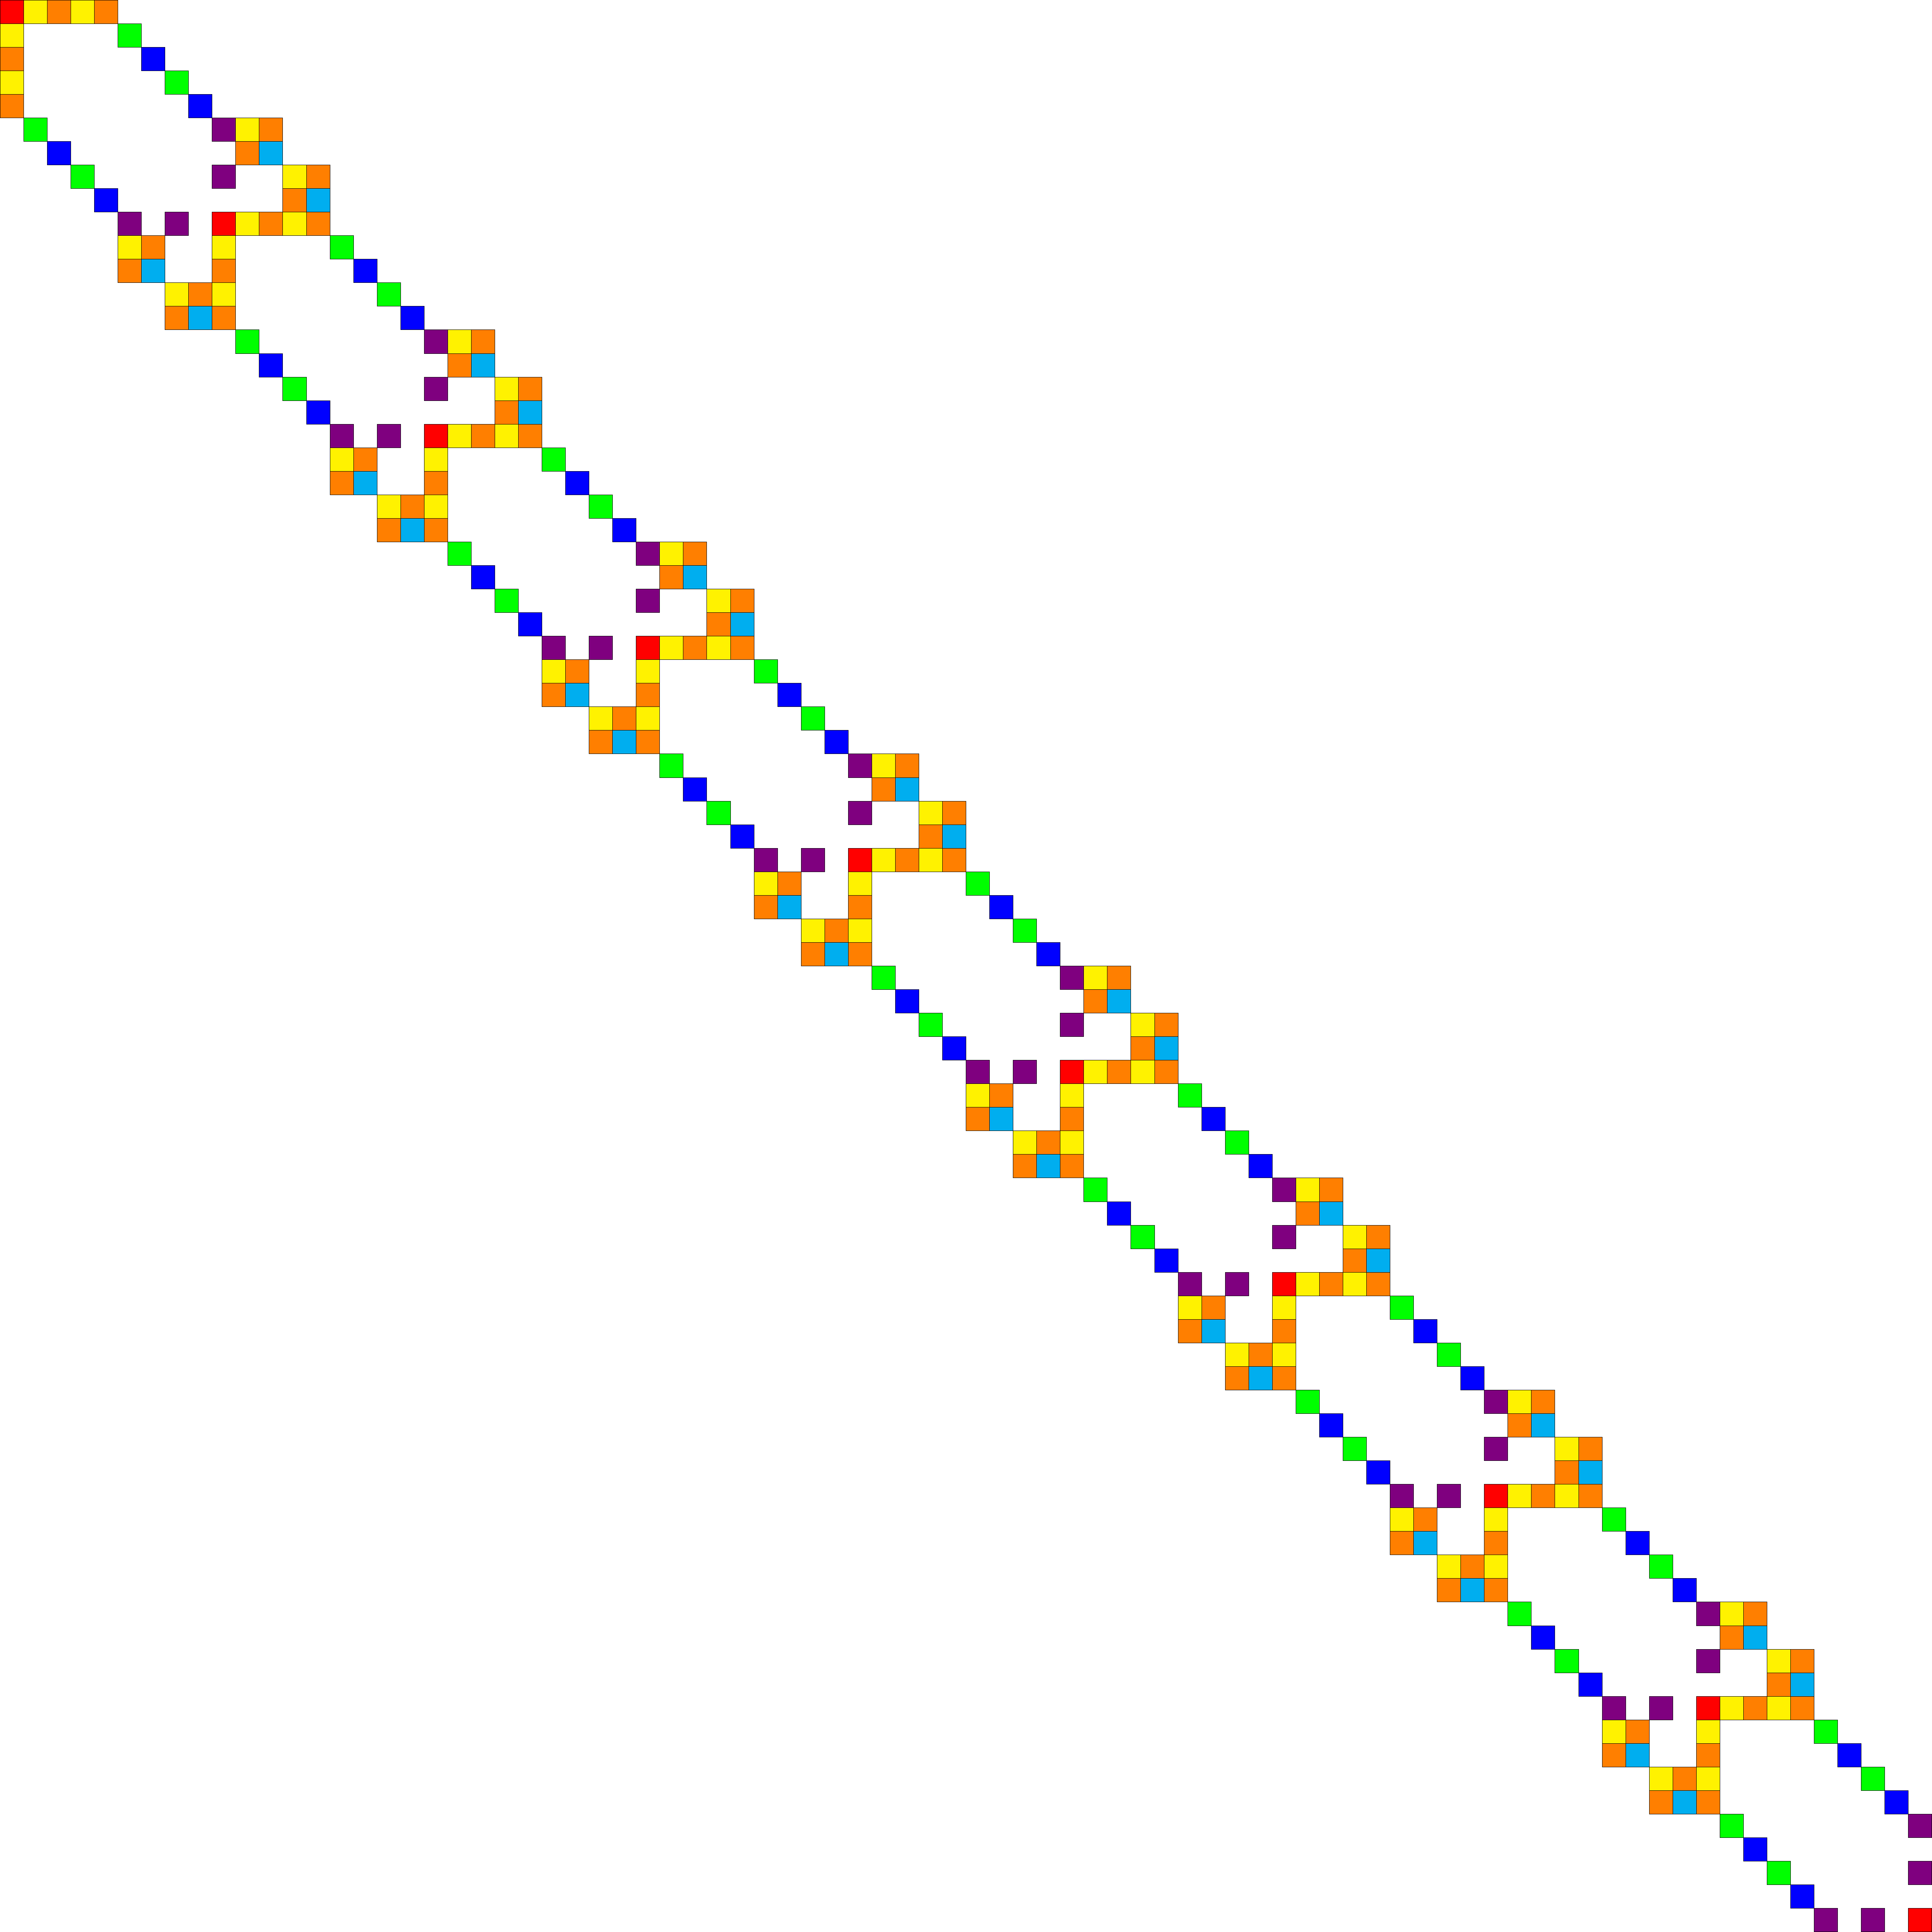
\includegraphics[scale=0.175]{./twoterm.eps}
\hspace{0.2in}
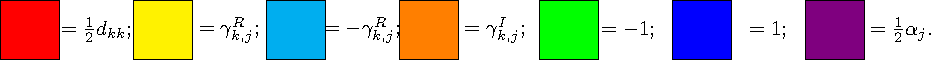
\includegraphics[scale=1.0]{./colorcode.eps}
\end{center}
\caption{Pictorial description of the extended sparse matrix where $N=10$, $p_0=0$, and $p=2$, following
the example shown in \citet{Ambikasaran2015}.}
\label{matrix_structure}
\end{figure}

{\bf Should I give some examples of this?  Some pseudocode?}

\bibliography{genrp}

\end{document}
